\documentclass{standalone}

%Til tikz billede
\usepackage{tikz}
\def\layersep{2.5cm}

\usetikzlibrary{shapes.multipart, matrix,chains,positioning,decorations.pathreplacing,shapes,arrows,arrows.meta}
\usetikzlibrary{arrows,decorations.pathmorphing,backgrounds,positioning,fit,petri}

% ggplot2 style tikz
\definecolor{trainFill}{gray}{0.95}
\definecolor{testFill}{gray}{0.80}
\definecolor{backG}{gray}{1}


\begin{document}
	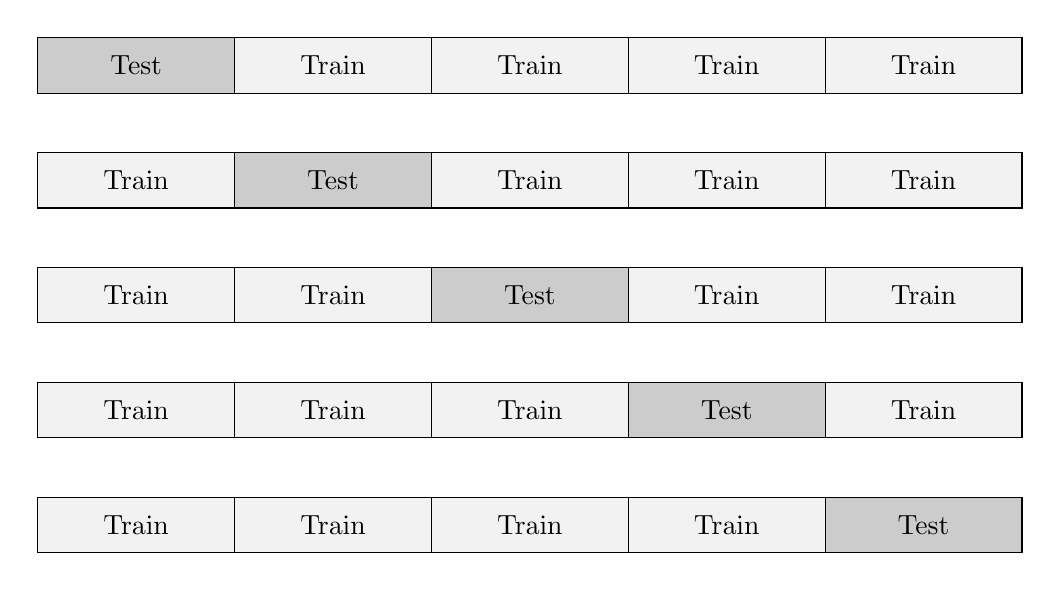
\begin{tikzpicture}[
	%  -{Stealth[length = 2.5pt]},
	start chain = going right,
	node distance = 0pt,
	train/.style={draw, minimum width=2.5cm, minimum height=2em, 
		outer sep=0pt, on chain, fill=trainFill},
	test/.style={draw, minimum width=2.5cm, minimum height=2em, 
		outer sep=0pt, on chain, fill=testFill},
	]
	\node [train] (1) at (0,0) {Train};
	\node [train] (2) {Train};
	\node [train] (3) {Train};
	\node [train] (4) {Train};
	\node [test] (5) {Test};
	\node [train, above=5ex of 1] (6) {Train};
	\node [train] (7) {Train};
	\node [train] (8) {Train};
	\node [test] (9) {Test};
	\node [train] (10) {Train};
	\node [train, above=5ex of 6] (11) {Train};
	\node [train] (12) {Train};
	\node [test] (13) {Test};
	\node [train] (14) {Train};
	\node [train] (15) {Train};
	\node [train, above=5ex of 11] (16) {Train};
	\node [test] (17) {Test};
	\node [train] (18) {Train};
	\node [train] (19) {Train};
	\node [train] (20) {Train};
	\node [test, above=5ex of 16] (21) {Test};
	\node [train] (22) {Train};
	\node [train] (23) {Train};
	\node [train] (24) {Train};
	\node [train] (25) {Train};
	
	
	\begin{pgfonlayer}{background}
	\node [fill=backG,fit=(current bounding box.north west) (current bounding box.south east)] {};
	\draw[step=1cm,white,very thin] (current bounding box.north west) grid (current bounding box.south east);
	\end{pgfonlayer}
	\end{tikzpicture}
\end{document}

 
